\documentclass{standalone}
\usepackage{tikz}
\usetikzlibrary{patterns, positioning}


\begin{document}
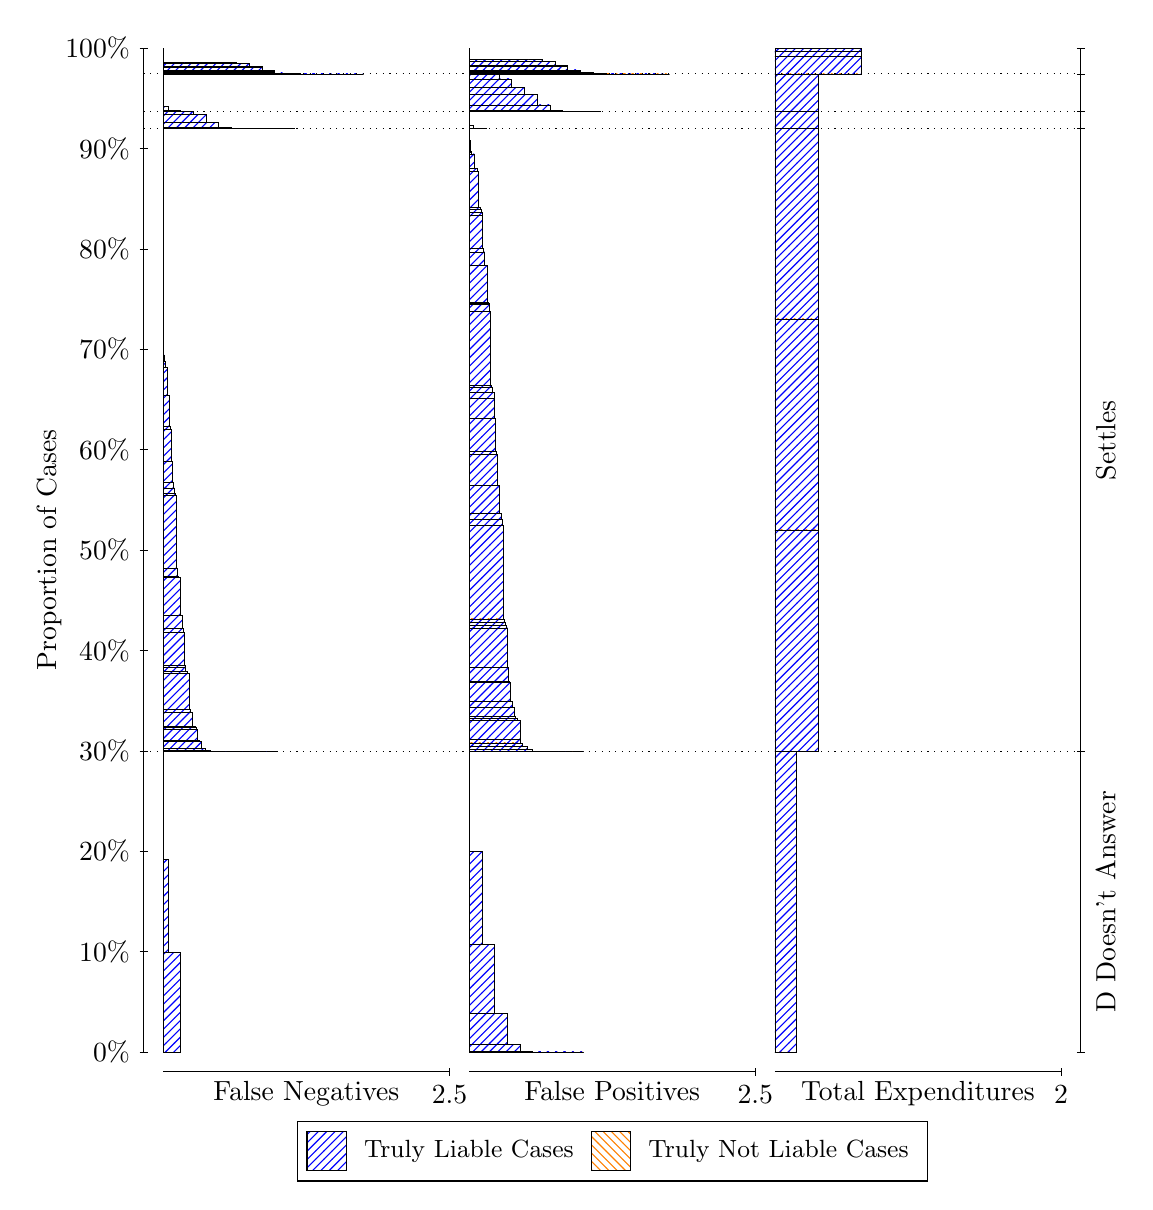
\begin{tikzpicture}
\draw[black, very thin] (1.5,1.75) -- (1.5,14.5);
\node[rotate=90, text=black, anchor=center] at (0.3, 8.125) {Proportion of Cases};
\draw[black, very thin] (1.45,1.75) -- (1.55,1.75);
\node[text=black, anchor=east] at (1.45, 1.75) {0\%};
\draw[black, very thin] (1.45,3.025) -- (1.55,3.025);
\node[text=black, anchor=east] at (1.45, 3.025) {10\%};
\draw[black, very thin] (1.45,4.3) -- (1.55,4.3);
\node[text=black, anchor=east] at (1.45, 4.3) {20\%};
\draw[black, very thin] (1.45,5.575) -- (1.55,5.575);
\node[text=black, anchor=east] at (1.45, 5.575) {30\%};
\draw[black, very thin] (1.45,6.85) -- (1.55,6.85);
\node[text=black, anchor=east] at (1.45, 6.85) {40\%};
\draw[black, very thin] (1.45,8.125) -- (1.55,8.125);
\node[text=black, anchor=east] at (1.45, 8.125) {50\%};
\draw[black, very thin] (1.45,9.4) -- (1.55,9.4);
\node[text=black, anchor=east] at (1.45, 9.4) {60\%};
\draw[black, very thin] (1.45,10.675) -- (1.55,10.675);
\node[text=black, anchor=east] at (1.45, 10.675) {70\%};
\draw[black, very thin] (1.45,11.95) -- (1.55,11.95);
\node[text=black, anchor=east] at (1.45, 11.95) {80\%};
\draw[black, very thin] (1.45,13.225) -- (1.55,13.225);
\node[text=black, anchor=east] at (1.45, 13.225) {90\%};
\draw[black, very thin] (1.45,14.5) -- (1.55,14.5);
\node[text=black, anchor=east] at (1.45, 14.5) {100\%};

\draw[black, very thin] (13.4,1.75) -- (13.4,14.5);
\draw[black, very thin] (13.35,1.75) -- (13.45,1.75);
\node[anchor=west] at (13.35, 1.75) {};
\draw[black, very thin] (13.35,5.5631) -- (13.45,5.5631);
\node[anchor=west] at (13.35, 5.5631) {};
\draw[black, very thin] (13.35,13.477) -- (13.45,13.477);
\node[anchor=west] at (13.35, 13.477) {};
\draw[black, very thin] (13.35,13.696) -- (13.45,13.696);
\node[anchor=west] at (13.35, 13.696) {};
\draw[black, very thin] (13.35,14.171) -- (13.45,14.171);
\node[anchor=west] at (13.35, 14.171) {};
\draw[black, very thin] (13.35,14.5) -- (13.45,14.5);
\node[anchor=west] at (13.35, 14.5) {};

\draw[black, very thin, pattern color=blue, pattern=north east lines] (1.75,1.75) rectangle (1.968,3.0136);
\draw[black, very thin, pattern color=blue, pattern=north east lines] (1.75,3.0136) rectangle (1.8065,4.1973);
\draw[black, very thin, pattern color=orange, pattern=north west lines] (1.75,4.1973) rectangle (1.75,4.1973);
\draw[black, very thin, pattern color=blue, pattern=north east lines] (1.75,4.1973) rectangle (1.75,5.5631);
\draw[black, very thin, pattern color=blue, pattern=north east lines] (1.75,5.5631) rectangle (3.2033,5.5631);
\draw[black, very thin, pattern color=blue, pattern=north east lines] (1.75,5.5631) rectangle (3.1307,5.5631);
\draw[black, very thin, pattern color=blue, pattern=north east lines] (1.75,5.5631) rectangle (3.058,5.5631);
\draw[black, very thin, pattern color=blue, pattern=north east lines] (1.75,5.5631) rectangle (3.0419,5.5631);
\draw[black, very thin, pattern color=blue, pattern=north east lines] (1.75,5.5631) rectangle (2.9853,5.5631);
\draw[black, very thin, pattern color=blue, pattern=north east lines] (1.75,5.5631) rectangle (2.9692,5.5631);
\draw[black, very thin, pattern color=blue, pattern=north east lines] (1.75,5.5631) rectangle (2.9127,5.5631);
\draw[black, very thin, pattern color=blue, pattern=north east lines] (1.75,5.5631) rectangle (2.8965,5.5631);
\draw[black, very thin, pattern color=blue, pattern=north east lines] (1.75,5.5631) rectangle (2.8804,5.5631);
\draw[black, very thin, pattern color=blue, pattern=north east lines] (1.75,5.5631) rectangle (2.84,5.5631);
\draw[black, very thin, pattern color=blue, pattern=north east lines] (1.75,5.5631) rectangle (2.8239,5.5631);
\draw[black, very thin, pattern color=blue, pattern=north east lines] (1.75,5.5631) rectangle (2.8077,5.5631);
\draw[black, very thin, pattern color=blue, pattern=north east lines] (1.75,5.5631) rectangle (2.7673,5.5631);
\draw[black, very thin, pattern color=blue, pattern=north east lines] (1.75,5.5631) rectangle (2.7512,5.5631);
\draw[black, very thin, pattern color=blue, pattern=north east lines] (1.75,5.5631) rectangle (2.735,5.5631);
\draw[black, very thin, pattern color=blue, pattern=north east lines] (1.75,5.5631) rectangle (2.7189,5.5631);
\draw[black, very thin, pattern color=blue, pattern=north east lines] (1.75,5.5631) rectangle (2.6947,5.5631);
\draw[black, very thin, pattern color=blue, pattern=north east lines] (1.75,5.5631) rectangle (2.6785,5.5631);
\draw[black, very thin, pattern color=blue, pattern=north east lines] (1.75,5.5631) rectangle (2.6624,5.5631);
\draw[black, very thin, pattern color=blue, pattern=north east lines] (1.75,5.5631) rectangle (2.6462,5.5631);
\draw[black, very thin, pattern color=blue, pattern=north east lines] (1.75,5.5631) rectangle (2.622,5.5631);
\draw[black, very thin, pattern color=blue, pattern=north east lines] (1.75,5.5631) rectangle (2.6059,5.5631);
\draw[black, very thin, pattern color=blue, pattern=north east lines] (1.75,5.5631) rectangle (2.5897,5.5631);
\draw[black, very thin, pattern color=blue, pattern=north east lines] (1.75,5.5631) rectangle (2.5736,5.5631);
\draw[black, very thin, pattern color=blue, pattern=north east lines] (1.75,5.5631) rectangle (2.5574,5.5632);
\draw[black, very thin, pattern color=blue, pattern=north east lines] (1.75,5.5632) rectangle (2.5493,5.5632);
\draw[black, very thin, pattern color=blue, pattern=north east lines] (1.75,5.5632) rectangle (2.5332,5.5632);
\draw[black, very thin, pattern color=blue, pattern=north east lines] (1.75,5.5632) rectangle (2.517,5.5632);
\draw[black, very thin, pattern color=blue, pattern=north east lines] (1.75,5.5632) rectangle (2.5009,5.5634);
\draw[black, very thin, pattern color=blue, pattern=north east lines] (1.75,5.5634) rectangle (2.4847,5.5634);
\draw[black, very thin, pattern color=blue, pattern=north east lines] (1.75,5.5634) rectangle (2.4767,5.5634);
\draw[black, very thin, pattern color=blue, pattern=north east lines] (1.75,5.5634) rectangle (2.4605,5.5634);
\draw[black, very thin, pattern color=blue, pattern=north east lines] (1.75,5.5634) rectangle (2.4444,5.5638);
\draw[black, very thin, pattern color=blue, pattern=north east lines] (1.75,5.5638) rectangle (2.4282,5.5638);
\draw[black, very thin, pattern color=blue, pattern=north east lines] (1.75,5.5638) rectangle (2.4121,5.5638);
\draw[black, very thin, pattern color=blue, pattern=north east lines] (1.75,5.5638) rectangle (2.3959,5.5703);
\draw[black, very thin, pattern color=blue, pattern=north east lines] (1.75,5.5703) rectangle (2.3879,5.5703);
\draw[black, very thin, pattern color=blue, pattern=north east lines] (1.75,5.5703) rectangle (2.3717,5.5703);
\draw[black, very thin, pattern color=blue, pattern=north east lines] (1.75,5.5703) rectangle (2.3556,5.5705);
\draw[black, very thin, pattern color=blue, pattern=north east lines] (1.75,5.5705) rectangle (2.3394,5.5829);
\draw[black, very thin, pattern color=blue, pattern=north east lines] (1.75,5.5829) rectangle (2.3313,5.5829);
\draw[black, very thin, pattern color=blue, pattern=north east lines] (1.75,5.5829) rectangle (2.3233,5.5846);
\draw[black, very thin, pattern color=blue, pattern=north east lines] (1.75,5.5846) rectangle (2.3152,5.585);
\draw[black, very thin, pattern color=blue, pattern=north east lines] (1.75,5.585) rectangle (2.299,5.585);
\draw[black, very thin, pattern color=blue, pattern=north east lines] (1.75,5.585) rectangle (2.2829,5.6016);
\draw[black, very thin, pattern color=blue, pattern=north east lines] (1.75,5.6016) rectangle (2.2667,5.6016);
\draw[black, very thin, pattern color=blue, pattern=north east lines] (1.75,5.6016) rectangle (2.2587,5.6016);
\draw[black, very thin, pattern color=blue, pattern=north east lines] (1.75,5.6016) rectangle (2.2506,5.605);
\draw[black, very thin, pattern color=blue, pattern=north east lines] (1.75,5.605) rectangle (2.2344,5.7012);
\draw[black, very thin, pattern color=blue, pattern=north east lines] (1.75,5.7012) rectangle (2.2264,5.7012);
\draw[black, very thin, pattern color=blue, pattern=north east lines] (1.75,5.7012) rectangle (2.2102,5.7036);
\draw[black, very thin, pattern color=blue, pattern=north east lines] (1.75,5.7036) rectangle (2.1941,5.7085);
\draw[black, very thin, pattern color=blue, pattern=north east lines] (1.75,5.7085) rectangle (2.186,5.7103);
\draw[black, very thin, pattern color=blue, pattern=north east lines] (1.75,5.7103) rectangle (2.1779,5.8493);
\draw[black, very thin, pattern color=blue, pattern=north east lines] (1.75,5.8493) rectangle (2.1699,5.8493);
\draw[black, very thin, pattern color=blue, pattern=north east lines] (1.75,5.8493) rectangle (2.1618,5.8678);
\draw[black, very thin, pattern color=blue, pattern=north east lines] (1.75,5.8678) rectangle (2.1537,5.8846);
\draw[black, very thin, pattern color=blue, pattern=north east lines] (1.75,5.8846) rectangle (2.1376,5.8846);
\draw[black, very thin, pattern color=blue, pattern=north east lines] (1.75,5.8846) rectangle (2.1214,6.0649);
\draw[black, very thin, pattern color=blue, pattern=north east lines] (1.75,6.0649) rectangle (2.1053,6.0659);
\draw[black, very thin, pattern color=blue, pattern=north east lines] (1.75,6.0659) rectangle (2.0972,6.0662);
\draw[black, very thin, pattern color=blue, pattern=north east lines] (1.75,6.0662) rectangle (2.0891,6.1031);
\draw[black, very thin, pattern color=blue, pattern=north east lines] (1.75,6.1031) rectangle (2.073,6.5588);
\draw[black, very thin, pattern color=blue, pattern=north east lines] (1.75,6.5588) rectangle (2.0649,6.5612);
\draw[black, very thin, pattern color=blue, pattern=north east lines] (1.75,6.5612) rectangle (2.0487,6.5886);
\draw[black, very thin, pattern color=blue, pattern=north east lines] (1.75,6.5886) rectangle (2.0326,6.6306);
\draw[black, very thin, pattern color=blue, pattern=north east lines] (1.75,6.6306) rectangle (2.0245,6.666);
\draw[black, very thin, pattern color=blue, pattern=north east lines] (1.75,6.666) rectangle (2.0164,7.0803);
\draw[black, very thin, pattern color=blue, pattern=north east lines] (1.75,7.0803) rectangle (2.0084,7.0803);
\draw[black, very thin, pattern color=blue, pattern=north east lines] (1.75,7.0803) rectangle (2.0003,7.129);
\draw[black, very thin, pattern color=blue, pattern=north east lines] (1.75,7.129) rectangle (1.9922,7.2967);
\draw[black, very thin, pattern color=blue, pattern=north east lines] (1.75,7.2967) rectangle (1.9761,7.297);
\draw[black, very thin, pattern color=blue, pattern=north east lines] (1.75,7.297) rectangle (1.9599,7.7754);
\draw[black, very thin, pattern color=blue, pattern=north east lines] (1.75,7.7754) rectangle (1.9438,7.7819);
\draw[black, very thin, pattern color=blue, pattern=north east lines] (1.75,7.7819) rectangle (1.9357,7.7911);
\draw[black, very thin, pattern color=blue, pattern=north east lines] (1.75,7.7911) rectangle (1.9276,7.8883);
\draw[black, very thin, pattern color=blue, pattern=north east lines] (1.75,7.8883) rectangle (1.9115,8.8224);
\draw[black, very thin, pattern color=blue, pattern=north east lines] (1.75,8.8224) rectangle (1.9034,8.8457);
\draw[black, very thin, pattern color=blue, pattern=north east lines] (1.75,8.8457) rectangle (1.8873,8.9146);
\draw[black, very thin, pattern color=blue, pattern=north east lines] (1.75,8.9146) rectangle (1.8711,8.9877);
\draw[black, very thin, pattern color=blue, pattern=north east lines] (1.75,8.9877) rectangle (1.863,9.2464);
\draw[black, very thin, pattern color=blue, pattern=north east lines] (1.75,9.2464) rectangle (1.855,9.6562);
\draw[black, very thin, pattern color=blue, pattern=north east lines] (1.75,9.6562) rectangle (1.8469,9.6568);
\draw[black, very thin, pattern color=blue, pattern=north east lines] (1.75,9.6568) rectangle (1.8388,9.6959);
\draw[black, very thin, pattern color=blue, pattern=north east lines] (1.75,9.6959) rectangle (1.8307,10.09);
\draw[black, very thin, pattern color=blue, pattern=north east lines] (1.75,10.09) rectangle (1.8146,10.092);
\draw[black, very thin, pattern color=blue, pattern=north east lines] (1.75,10.092) rectangle (1.7984,10.444);
\draw[black, very thin, pattern color=blue, pattern=north east lines] (1.75,10.444) rectangle (1.7823,10.451);
\draw[black, very thin, pattern color=blue, pattern=north east lines] (1.75,10.451) rectangle (1.7742,10.526);
\draw[black, very thin, pattern color=blue, pattern=north east lines] (1.75,10.526) rectangle (1.7661,10.604);
\draw[black, very thin, pattern color=orange, pattern=north west lines] (1.75,10.604) rectangle (1.75,10.604);
\draw[black, very thin, pattern color=blue, pattern=north east lines] (1.75,10.604) rectangle (1.75,13.477);
\draw[black, very thin, pattern color=blue, pattern=north east lines] (1.75,13.477) rectangle (3.4213,13.477);
\draw[black, very thin, pattern color=blue, pattern=north east lines] (1.75,13.477) rectangle (3.2599,13.477);
\draw[black, very thin, pattern color=blue, pattern=north east lines] (1.75,13.477) rectangle (3.0984,13.477);
\draw[black, very thin, pattern color=blue, pattern=north east lines] (1.75,13.477) rectangle (2.9369,13.477);
\draw[black, very thin, pattern color=blue, pattern=north east lines] (1.75,13.477) rectangle (2.7754,13.477);
\draw[black, very thin, pattern color=blue, pattern=north east lines] (1.75,13.477) rectangle (2.6139,13.488);
\draw[black, very thin, pattern color=blue, pattern=north east lines] (1.75,13.488) rectangle (2.4524,13.555);
\draw[black, very thin, pattern color=blue, pattern=north east lines] (1.75,13.555) rectangle (2.291,13.653);
\draw[black, very thin, pattern color=blue, pattern=north east lines] (1.75,13.653) rectangle (2.1295,13.691);
\draw[black, very thin, pattern color=blue, pattern=north east lines] (1.75,13.691) rectangle (1.968,13.696);
\draw[black, very thin, pattern color=orange, pattern=north west lines] (1.75,13.696) rectangle (1.75,13.696);
\draw[black, very thin, pattern color=blue, pattern=north east lines] (1.75,13.696) rectangle (1.968,13.706);
\draw[black, very thin, pattern color=blue, pattern=north east lines] (1.75,13.706) rectangle (1.8065,13.76);
\draw[black, very thin, pattern color=orange, pattern=north west lines] (1.75,13.76) rectangle (1.75,13.76);
\draw[black, very thin, pattern color=blue, pattern=north east lines] (1.75,13.76) rectangle (1.75,14.171);
\draw[black, very thin, pattern color=blue, pattern=north east lines] (1.75,14.171) rectangle (4.2933,14.171);
\draw[black, very thin, pattern color=blue, pattern=north east lines] (1.75,14.171) rectangle (4.1319,14.171);
\draw[black, very thin, pattern color=blue, pattern=north east lines] (1.75,14.171) rectangle (3.9704,14.171);
\draw[black, very thin, pattern color=blue, pattern=north east lines] (1.75,14.171) rectangle (3.8089,14.171);
\draw[black, very thin, pattern color=blue, pattern=north east lines] (1.75,14.171) rectangle (3.8089,14.171);
\draw[black, very thin, pattern color=blue, pattern=north east lines] (1.75,14.171) rectangle (3.6474,14.171);
\draw[black, very thin, pattern color=blue, pattern=north east lines] (1.75,14.171) rectangle (3.6474,14.171);
\draw[black, very thin, pattern color=blue, pattern=north east lines] (1.75,14.171) rectangle (3.4859,14.173);
\draw[black, very thin, pattern color=blue, pattern=north east lines] (1.75,14.173) rectangle (3.3244,14.175);
\draw[black, very thin, pattern color=blue, pattern=north east lines] (1.75,14.175) rectangle (3.3244,14.183);
\draw[black, very thin, pattern color=blue, pattern=north east lines] (1.75,14.183) rectangle (3.163,14.188);
\draw[black, very thin, pattern color=blue, pattern=north east lines] (1.75,14.188) rectangle (3.163,14.205);
\draw[black, very thin, pattern color=blue, pattern=north east lines] (1.75,14.205) rectangle (3.163,14.216);
\draw[black, very thin, pattern color=blue, pattern=north east lines] (1.75,14.216) rectangle (3.0015,14.254);
\draw[black, very thin, pattern color=blue, pattern=north east lines] (1.75,14.254) rectangle (3.0015,14.266);
\draw[black, very thin, pattern color=blue, pattern=north east lines] (1.75,14.266) rectangle (2.84,14.303);
\draw[black, very thin, pattern color=blue, pattern=north east lines] (1.75,14.303) rectangle (2.6785,14.305);
\draw[black, very thin, pattern color=blue, pattern=north east lines] (1.75,14.305) rectangle (2.6785,14.313);
\draw[black, very thin, pattern color=blue, pattern=north east lines] (1.75,14.313) rectangle (2.6624,14.313);
\draw[black, very thin, pattern color=blue, pattern=north east lines] (1.75,14.313) rectangle (2.517,14.313);
\draw[black, very thin, pattern color=blue, pattern=north east lines] (1.75,14.313) rectangle (2.517,14.313);
\draw[black, very thin, pattern color=blue, pattern=north east lines] (1.75,14.313) rectangle (2.5009,14.313);
\draw[black, very thin, pattern color=blue, pattern=north east lines] (1.75,14.313) rectangle (2.5009,14.313);
\draw[black, very thin, pattern color=blue, pattern=north east lines] (1.75,14.313) rectangle (2.3556,14.313);
\draw[black, very thin, pattern color=blue, pattern=north east lines] (1.75,14.313) rectangle (2.3556,14.313);
\draw[black, very thin, pattern color=blue, pattern=north east lines] (1.75,14.313) rectangle (2.3394,14.313);
\draw[black, very thin, pattern color=blue, pattern=north east lines] (1.75,14.313) rectangle (2.3394,14.313);
\draw[black, very thin, pattern color=blue, pattern=north east lines] (1.75,14.313) rectangle (2.3394,14.313);
\draw[black, very thin, pattern color=blue, pattern=north east lines] (1.75,14.313) rectangle (2.1941,14.313);
\draw[black, very thin, pattern color=blue, pattern=north east lines] (1.75,14.313) rectangle (2.1941,14.313);
\draw[black, very thin, pattern color=blue, pattern=north east lines] (1.75,14.313) rectangle (2.1779,14.313);
\draw[black, very thin, pattern color=blue, pattern=north east lines] (1.75,14.313) rectangle (2.1779,14.313);
\draw[black, very thin, pattern color=blue, pattern=north east lines] (1.75,14.313) rectangle (2.0326,14.313);
\draw[black, very thin, pattern color=blue, pattern=north east lines] (1.75,14.313) rectangle (2.0326,14.313);
\draw[black, very thin, pattern color=blue, pattern=north east lines] (1.75,14.313) rectangle (2.0164,14.313);
\draw[black, very thin, pattern color=blue, pattern=north east lines] (1.75,14.313) rectangle (2.0164,14.313);
\draw[black, very thin, pattern color=blue, pattern=north east lines] (1.75,14.313) rectangle (2.0164,14.313);
\draw[black, very thin, pattern color=blue, pattern=north east lines] (1.75,14.313) rectangle (1.8711,14.313);
\draw[black, very thin, pattern color=blue, pattern=north east lines] (1.75,14.313) rectangle (1.8711,14.313);
\draw[black, very thin, pattern color=blue, pattern=north east lines] (1.75,14.313) rectangle (1.855,14.314);
\draw[black, very thin, pattern color=blue, pattern=north east lines] (1.75,14.314) rectangle (1.855,14.316);
\draw[black, very thin, pattern color=blue, pattern=north east lines] (1.75,14.316) rectangle (1.855,14.316);
\draw[black, very thin, pattern color=orange, pattern=north west lines] (1.75,14.316) rectangle (1.75,14.316);
\draw[black, very thin, pattern color=blue, pattern=north east lines] (1.75,14.316) rectangle (1.75,14.5);
\draw[black, very thin, pattern color=orange, pattern=north west lines] (5.6333,1.75) rectangle (7.0867,1.75);
\draw[black, very thin, pattern color=blue, pattern=north east lines] (5.6333,1.75) rectangle (7.0867,1.75);
\draw[black, very thin, pattern color=blue, pattern=north east lines] (5.6333,1.75) rectangle (6.9252,1.75);
\draw[black, very thin, pattern color=blue, pattern=north east lines] (5.6333,1.75) rectangle (6.7637,1.75);
\draw[black, very thin, pattern color=blue, pattern=north east lines] (5.6333,1.75) rectangle (6.6022,1.7503);
\draw[black, very thin, pattern color=blue, pattern=north east lines] (5.6333,1.7503) rectangle (6.4407,1.7582);
\draw[black, very thin, pattern color=blue, pattern=north east lines] (5.6333,1.7582) rectangle (6.2793,1.8434);
\draw[black, very thin, pattern color=blue, pattern=north east lines] (5.6333,1.8434) rectangle (6.1178,2.2366);
\draw[black, very thin, pattern color=blue, pattern=north east lines] (5.6333,2.2366) rectangle (5.9563,3.1157);
\draw[black, very thin, pattern color=blue, pattern=north east lines] (5.6333,3.1157) rectangle (5.7948,4.2995);
\draw[black, very thin, pattern color=blue, pattern=north east lines] (5.6333,4.2995) rectangle (5.6333,5.5631);
\draw[black, very thin, pattern color=orange, pattern=north west lines] (5.6333,5.5631) rectangle (7.0867,5.5631);
\draw[black, very thin, pattern color=blue, pattern=north east lines] (5.6333,5.5631) rectangle (7.0867,5.5631);
\draw[black, very thin, pattern color=orange, pattern=north west lines] (5.6333,5.5631) rectangle (7.014,5.5631);
\draw[black, very thin, pattern color=blue, pattern=north east lines] (5.6333,5.5631) rectangle (7.014,5.5631);
\draw[black, very thin, pattern color=orange, pattern=north west lines] (5.6333,5.5631) rectangle (6.9413,5.5631);
\draw[black, very thin, pattern color=blue, pattern=north east lines] (5.6333,5.5631) rectangle (6.9413,5.5631);
\draw[black, very thin, pattern color=blue, pattern=north east lines] (5.6333,5.5631) rectangle (6.9252,5.5631);
\draw[black, very thin, pattern color=blue, pattern=north east lines] (5.6333,5.5631) rectangle (6.8525,5.5631);
\draw[black, very thin, pattern color=orange, pattern=north west lines] (5.6333,5.5631) rectangle (6.796,5.5631);
\draw[black, very thin, pattern color=blue, pattern=north east lines] (5.6333,5.5631) rectangle (6.796,5.5631);
\draw[black, very thin, pattern color=blue, pattern=north east lines] (5.6333,5.5631) rectangle (6.7799,5.5631);
\draw[black, very thin, pattern color=blue, pattern=north east lines] (5.6333,5.5631) rectangle (6.7637,5.5631);
\draw[black, very thin, pattern color=orange, pattern=north west lines] (5.6333,5.5631) rectangle (6.7233,5.5631);
\draw[black, very thin, pattern color=blue, pattern=north east lines] (5.6333,5.5631) rectangle (6.7233,5.5631);
\draw[black, very thin, pattern color=blue, pattern=north east lines] (5.6333,5.5631) rectangle (6.691,5.5631);
\draw[black, very thin, pattern color=orange, pattern=north west lines] (5.6333,5.5631) rectangle (6.6507,5.5631);
\draw[black, very thin, pattern color=blue, pattern=north east lines] (5.6333,5.5631) rectangle (6.6507,5.5631);
\draw[black, very thin, pattern color=blue, pattern=north east lines] (5.6333,5.5631) rectangle (6.6345,5.5631);
\draw[black, very thin, pattern color=blue, pattern=north east lines] (5.6333,5.5631) rectangle (6.6184,5.5631);
\draw[black, very thin, pattern color=blue, pattern=north east lines] (5.6333,5.5631) rectangle (6.6022,5.5636);
\draw[black, very thin, pattern color=orange, pattern=north west lines] (5.6333,5.5636) rectangle (6.578,5.5636);
\draw[black, very thin, pattern color=blue, pattern=north east lines] (5.6333,5.5636) rectangle (6.578,5.5636);
\draw[black, very thin, pattern color=blue, pattern=north east lines] (5.6333,5.5636) rectangle (6.5619,5.5637);
\draw[black, very thin, pattern color=blue, pattern=north east lines] (5.6333,5.5637) rectangle (6.5296,5.5657);
\draw[black, very thin, pattern color=orange, pattern=north west lines] (5.6333,5.5657) rectangle (6.5053,5.5657);
\draw[black, very thin, pattern color=blue, pattern=north east lines] (5.6333,5.5657) rectangle (6.5053,5.5658);
\draw[black, very thin, pattern color=blue, pattern=north east lines] (5.6333,5.5658) rectangle (6.4892,5.5658);
\draw[black, very thin, pattern color=blue, pattern=north east lines] (5.6333,5.5658) rectangle (6.473,5.5669);
\draw[black, very thin, pattern color=blue, pattern=north east lines] (5.6333,5.5669) rectangle (6.4569,5.5675);
\draw[black, very thin, pattern color=blue, pattern=north east lines] (5.6333,5.5675) rectangle (6.4407,5.5932);
\draw[black, very thin, pattern color=orange, pattern=north west lines] (5.6333,5.5932) rectangle (6.4327,5.5932);
\draw[black, very thin, pattern color=blue, pattern=north east lines] (5.6333,5.5932) rectangle (6.4327,5.5933);
\draw[black, very thin, pattern color=blue, pattern=north east lines] (5.6333,5.5933) rectangle (6.4165,5.5936);
\draw[black, very thin, pattern color=blue, pattern=north east lines] (5.6333,5.5936) rectangle (6.4004,5.5949);
\draw[black, very thin, pattern color=blue, pattern=north east lines] (5.6333,5.5949) rectangle (6.3681,5.6311);
\draw[black, very thin, pattern color=orange, pattern=north west lines] (5.6333,5.6311) rectangle (6.36,5.6311);
\draw[black, very thin, pattern color=blue, pattern=north east lines] (5.6333,5.6311) rectangle (6.36,5.6311);
\draw[black, very thin, pattern color=blue, pattern=north east lines] (5.6333,5.6311) rectangle (6.3439,5.6365);
\draw[black, very thin, pattern color=blue, pattern=north east lines] (5.6333,5.6365) rectangle (6.3277,5.6368);
\draw[black, very thin, pattern color=blue, pattern=north east lines] (5.6333,5.6368) rectangle (6.3116,5.6707);
\draw[black, very thin, pattern color=blue, pattern=north east lines] (5.6333,5.6707) rectangle (6.2954,5.6744);
\draw[black, very thin, pattern color=orange, pattern=north west lines] (5.6333,5.6744) rectangle (6.2873,5.6744);
\draw[black, very thin, pattern color=blue, pattern=north east lines] (5.6333,5.6744) rectangle (6.2873,5.715);
\draw[black, very thin, pattern color=blue, pattern=north east lines] (5.6333,5.715) rectangle (6.2793,5.9566);
\draw[black, very thin, pattern color=blue, pattern=north east lines] (5.6333,5.9566) rectangle (6.2712,5.9591);
\draw[black, very thin, pattern color=blue, pattern=north east lines] (5.6333,5.9591) rectangle (6.255,5.9655);
\draw[black, very thin, pattern color=blue, pattern=north east lines] (5.6333,5.9655) rectangle (6.2389,5.9828);
\draw[black, very thin, pattern color=orange, pattern=north west lines] (5.6333,5.9828) rectangle (6.2147,5.9828);
\draw[black, very thin, pattern color=blue, pattern=north east lines] (5.6333,5.9828) rectangle (6.2147,6.0102);
\draw[black, very thin, pattern color=blue, pattern=north east lines] (5.6333,6.0102) rectangle (6.2066,6.1285);
\draw[black, very thin, pattern color=blue, pattern=north east lines] (5.6333,6.1285) rectangle (6.1985,6.1297);
\draw[black, very thin, pattern color=blue, pattern=north east lines] (5.6333,6.1297) rectangle (6.1824,6.2066);
\draw[black, very thin, pattern color=blue, pattern=north east lines] (5.6333,6.2066) rectangle (6.1662,6.2088);
\draw[black, very thin, pattern color=blue, pattern=north east lines] (5.6333,6.2088) rectangle (6.1501,6.4425);
\draw[black, very thin, pattern color=orange, pattern=north west lines] (5.6333,6.4425) rectangle (6.142,6.4425);
\draw[black, very thin, pattern color=blue, pattern=north east lines] (5.6333,6.4425) rectangle (6.142,6.4563);
\draw[black, very thin, pattern color=blue, pattern=north east lines] (5.6333,6.4563) rectangle (6.1339,6.46);
\draw[black, very thin, pattern color=blue, pattern=north east lines] (5.6333,6.46) rectangle (6.1259,6.6298);
\draw[black, very thin, pattern color=blue, pattern=north east lines] (5.6333,6.6298) rectangle (6.1178,7.1352);
\draw[black, very thin, pattern color=blue, pattern=north east lines] (5.6333,7.1352) rectangle (6.1097,7.163);
\draw[black, very thin, pattern color=blue, pattern=north east lines] (5.6333,7.163) rectangle (6.0936,7.2043);
\draw[black, very thin, pattern color=blue, pattern=north east lines] (5.6333,7.2043) rectangle (6.0774,7.2492);
\draw[black, very thin, pattern color=orange, pattern=north west lines] (5.6333,7.2492) rectangle (6.0693,7.2492);
\draw[black, very thin, pattern color=blue, pattern=north east lines] (5.6333,7.2492) rectangle (6.0693,8.4361);
\draw[black, very thin, pattern color=blue, pattern=north east lines] (5.6333,8.4361) rectangle (6.0532,8.5142);
\draw[black, very thin, pattern color=blue, pattern=north east lines] (5.6333,8.5142) rectangle (6.0451,8.5889);
\draw[black, very thin, pattern color=blue, pattern=north east lines] (5.6333,8.5889) rectangle (6.037,8.5955);
\draw[black, very thin, pattern color=blue, pattern=north east lines] (5.6333,8.5955) rectangle (6.0209,8.9475);
\draw[black, very thin, pattern color=blue, pattern=north east lines] (5.6333,8.9475) rectangle (6.0047,8.9497);
\draw[black, very thin, pattern color=blue, pattern=north east lines] (5.6333,8.9497) rectangle (5.9886,9.344);
\draw[black, very thin, pattern color=blue, pattern=north east lines] (5.6333,9.344) rectangle (5.9805,9.3831);
\draw[black, very thin, pattern color=blue, pattern=north east lines] (5.6333,9.3831) rectangle (5.9724,9.3837);
\draw[black, very thin, pattern color=blue, pattern=north east lines] (5.6333,9.3837) rectangle (5.9644,9.7935);
\draw[black, very thin, pattern color=blue, pattern=north east lines] (5.6333,9.7935) rectangle (5.9563,10.052);
\draw[black, very thin, pattern color=blue, pattern=north east lines] (5.6333,10.052) rectangle (5.9482,10.125);
\draw[black, very thin, pattern color=blue, pattern=north east lines] (5.6333,10.125) rectangle (5.9321,10.194);
\draw[black, very thin, pattern color=blue, pattern=north east lines] (5.6333,10.194) rectangle (5.9159,10.217);
\draw[black, very thin, pattern color=blue, pattern=north east lines] (5.6333,10.217) rectangle (5.9079,11.152);
\draw[black, very thin, pattern color=blue, pattern=north east lines] (5.6333,11.152) rectangle (5.8917,11.249);
\draw[black, very thin, pattern color=blue, pattern=north east lines] (5.6333,11.249) rectangle (5.8836,11.258);
\draw[black, very thin, pattern color=blue, pattern=north east lines] (5.6333,11.258) rectangle (5.8756,11.265);
\draw[black, very thin, pattern color=blue, pattern=north east lines] (5.6333,11.265) rectangle (5.8594,11.743);
\draw[black, very thin, pattern color=blue, pattern=north east lines] (5.6333,11.743) rectangle (5.8433,11.743);
\draw[black, very thin, pattern color=blue, pattern=north east lines] (5.6333,11.743) rectangle (5.8271,11.911);
\draw[black, very thin, pattern color=blue, pattern=north east lines] (5.6333,11.911) rectangle (5.819,11.96);
\draw[black, very thin, pattern color=blue, pattern=north east lines] (5.6333,11.96) rectangle (5.811,11.96);
\draw[black, very thin, pattern color=blue, pattern=north east lines] (5.6333,11.96) rectangle (5.8029,12.374);
\draw[black, very thin, pattern color=blue, pattern=north east lines] (5.6333,12.374) rectangle (5.7948,12.409);
\draw[black, very thin, pattern color=blue, pattern=north east lines] (5.6333,12.409) rectangle (5.7867,12.451);
\draw[black, very thin, pattern color=blue, pattern=north east lines] (5.6333,12.451) rectangle (5.7706,12.479);
\draw[black, very thin, pattern color=blue, pattern=north east lines] (5.6333,12.479) rectangle (5.7544,12.481);
\draw[black, very thin, pattern color=blue, pattern=north east lines] (5.6333,12.481) rectangle (5.7464,12.937);
\draw[black, very thin, pattern color=blue, pattern=north east lines] (5.6333,12.937) rectangle (5.7302,12.974);
\draw[black, very thin, pattern color=blue, pattern=north east lines] (5.6333,12.974) rectangle (5.7221,12.974);
\draw[black, very thin, pattern color=blue, pattern=north east lines] (5.6333,12.974) rectangle (5.7141,12.975);
\draw[black, very thin, pattern color=blue, pattern=north east lines] (5.6333,12.975) rectangle (5.6979,13.155);
\draw[black, very thin, pattern color=blue, pattern=north east lines] (5.6333,13.155) rectangle (5.6818,13.155);
\draw[black, very thin, pattern color=blue, pattern=north east lines] (5.6333,13.155) rectangle (5.6656,13.172);
\draw[black, very thin, pattern color=blue, pattern=north east lines] (5.6333,13.172) rectangle (5.6576,13.191);
\draw[black, very thin, pattern color=blue, pattern=north east lines] (5.6333,13.191) rectangle (5.6495,13.191);
\draw[black, very thin, pattern color=blue, pattern=north east lines] (5.6333,13.191) rectangle (5.6414,13.33);
\draw[black, very thin, pattern color=blue, pattern=north east lines] (5.6333,13.33) rectangle (5.6333,13.477);
\draw[black, very thin, pattern color=orange, pattern=north west lines] (5.6333,13.477) rectangle (5.8513,13.477);
\draw[black, very thin, pattern color=blue, pattern=north east lines] (5.6333,13.477) rectangle (5.8513,13.483);
\draw[black, very thin, pattern color=blue, pattern=north east lines] (5.6333,13.483) rectangle (5.6899,13.521);
\draw[black, very thin, pattern color=blue, pattern=north east lines] (5.6333,13.521) rectangle (5.6333,13.696);
\draw[black, very thin, pattern color=orange, pattern=north west lines] (5.6333,13.696) rectangle (7.3047,13.696);
\draw[black, very thin, pattern color=blue, pattern=north east lines] (5.6333,13.696) rectangle (7.3047,13.696);
\draw[black, very thin, pattern color=blue, pattern=north east lines] (5.6333,13.696) rectangle (7.1432,13.696);
\draw[black, very thin, pattern color=blue, pattern=north east lines] (5.6333,13.696) rectangle (6.9817,13.697);
\draw[black, very thin, pattern color=blue, pattern=north east lines] (5.6333,13.697) rectangle (6.8202,13.705);
\draw[black, very thin, pattern color=blue, pattern=north east lines] (5.6333,13.705) rectangle (6.6587,13.777);
\draw[black, very thin, pattern color=blue, pattern=north east lines] (5.6333,13.777) rectangle (6.4973,13.91);
\draw[black, very thin, pattern color=blue, pattern=north east lines] (5.6333,13.91) rectangle (6.3358,14.005);
\draw[black, very thin, pattern color=blue, pattern=north east lines] (5.6333,14.005) rectangle (6.1743,14.108);
\draw[black, very thin, pattern color=blue, pattern=north east lines] (5.6333,14.108) rectangle (6.0128,14.162);
\draw[black, very thin, pattern color=blue, pattern=north east lines] (5.6333,14.162) rectangle (5.8513,14.171);
\draw[black, very thin, pattern color=orange, pattern=north west lines] (5.6333,14.171) rectangle (8.1767,14.171);
\draw[black, very thin, pattern color=blue, pattern=north east lines] (5.6333,14.171) rectangle (8.1767,14.171);
\draw[black, very thin, pattern color=orange, pattern=north west lines] (5.6333,14.171) rectangle (8.0152,14.171);
\draw[black, very thin, pattern color=blue, pattern=north east lines] (5.6333,14.171) rectangle (8.0152,14.171);
\draw[black, very thin, pattern color=orange, pattern=north west lines] (5.6333,14.171) rectangle (7.8537,14.171);
\draw[black, very thin, pattern color=blue, pattern=north east lines] (5.6333,14.171) rectangle (7.8537,14.171);
\draw[black, very thin, pattern color=blue, pattern=north east lines] (5.6333,14.171) rectangle (7.6922,14.171);
\draw[black, very thin, pattern color=orange, pattern=north west lines] (5.6333,14.171) rectangle (7.6922,14.171);
\draw[black, very thin, pattern color=blue, pattern=north east lines] (5.6333,14.171) rectangle (7.6922,14.171);
\draw[black, very thin, pattern color=orange, pattern=north west lines] (5.6333,14.171) rectangle (7.5307,14.171);
\draw[black, very thin, pattern color=blue, pattern=north east lines] (5.6333,14.171) rectangle (7.5307,14.171);
\draw[black, very thin, pattern color=blue, pattern=north east lines] (5.6333,14.171) rectangle (7.5307,14.171);
\draw[black, very thin, pattern color=orange, pattern=north west lines] (5.6333,14.171) rectangle (7.3693,14.171);
\draw[black, very thin, pattern color=blue, pattern=north east lines] (5.6333,14.171) rectangle (7.3693,14.174);
\draw[black, very thin, pattern color=blue, pattern=north east lines] (5.6333,14.174) rectangle (7.3693,14.174);
\draw[black, very thin, pattern color=blue, pattern=north east lines] (5.6333,14.174) rectangle (7.2078,14.176);
\draw[black, very thin, pattern color=orange, pattern=north west lines] (5.6333,14.176) rectangle (7.2078,14.176);
\draw[black, very thin, pattern color=blue, pattern=north east lines] (5.6333,14.176) rectangle (7.2078,14.186);
\draw[black, very thin, pattern color=blue, pattern=north east lines] (5.6333,14.186) rectangle (7.0463,14.198);
\draw[black, very thin, pattern color=orange, pattern=north west lines] (5.6333,14.198) rectangle (7.0463,14.198);
\draw[black, very thin, pattern color=blue, pattern=north east lines] (5.6333,14.198) rectangle (7.0463,14.206);
\draw[black, very thin, pattern color=blue, pattern=north east lines] (5.6333,14.206) rectangle (7.0463,14.223);
\draw[black, very thin, pattern color=blue, pattern=north east lines] (5.6333,14.223) rectangle (6.8848,14.263);
\draw[black, very thin, pattern color=blue, pattern=north east lines] (5.6333,14.263) rectangle (6.8848,14.275);
\draw[black, very thin, pattern color=blue, pattern=north east lines] (5.6333,14.275) rectangle (6.8848,14.284);
\draw[black, very thin, pattern color=blue, pattern=north east lines] (5.6333,14.284) rectangle (6.7233,14.332);
\draw[black, very thin, pattern color=blue, pattern=north east lines] (5.6333,14.332) rectangle (6.7233,14.334);
\draw[black, very thin, pattern color=blue, pattern=north east lines] (5.6333,14.334) rectangle (6.5619,14.336);
\draw[black, very thin, pattern color=blue, pattern=north east lines] (5.6333,14.336) rectangle (6.5619,14.355);
\draw[black, very thin, pattern color=blue, pattern=north east lines] (5.6333,14.355) rectangle (6.5619,14.355);
\draw[black, very thin, pattern color=orange, pattern=north west lines] (5.6333,14.355) rectangle (6.5457,14.355);
\draw[black, very thin, pattern color=blue, pattern=north east lines] (5.6333,14.355) rectangle (6.5457,14.355);
\draw[black, very thin, pattern color=blue, pattern=north east lines] (5.6333,14.355) rectangle (6.4004,14.357);
\draw[black, very thin, pattern color=blue, pattern=north east lines] (5.6333,14.357) rectangle (6.4004,14.358);
\draw[black, very thin, pattern color=orange, pattern=north west lines] (5.6333,14.358) rectangle (6.3842,14.358);
\draw[black, very thin, pattern color=blue, pattern=north east lines] (5.6333,14.358) rectangle (6.3842,14.358);
\draw[black, very thin, pattern color=blue, pattern=north east lines] (5.6333,14.358) rectangle (6.2389,14.358);
\draw[black, very thin, pattern color=blue, pattern=north east lines] (5.6333,14.358) rectangle (6.2389,14.358);
\draw[black, very thin, pattern color=blue, pattern=north east lines] (5.6333,14.358) rectangle (6.2389,14.358);
\draw[black, very thin, pattern color=orange, pattern=north west lines] (5.6333,14.358) rectangle (6.2227,14.358);
\draw[black, very thin, pattern color=blue, pattern=north east lines] (5.6333,14.358) rectangle (6.2227,14.358);
\draw[black, very thin, pattern color=blue, pattern=north east lines] (5.6333,14.358) rectangle (6.2227,14.358);
\draw[black, very thin, pattern color=blue, pattern=north east lines] (5.6333,14.358) rectangle (6.2227,14.358);
\draw[black, very thin, pattern color=blue, pattern=north east lines] (5.6333,14.358) rectangle (6.0774,14.358);
\draw[black, very thin, pattern color=blue, pattern=north east lines] (5.6333,14.358) rectangle (6.0774,14.358);
\draw[black, very thin, pattern color=blue, pattern=north east lines] (5.6333,14.358) rectangle (6.0613,14.358);
\draw[black, very thin, pattern color=orange, pattern=north west lines] (5.6333,14.358) rectangle (6.0613,14.358);
\draw[black, very thin, pattern color=blue, pattern=north east lines] (5.6333,14.358) rectangle (6.0613,14.358);
\draw[black, very thin, pattern color=blue, pattern=north east lines] (5.6333,14.358) rectangle (6.0613,14.358);
\draw[black, very thin, pattern color=blue, pattern=north east lines] (5.6333,14.358) rectangle (5.9159,14.358);
\draw[black, very thin, pattern color=blue, pattern=north east lines] (5.6333,14.358) rectangle (5.8998,14.358);
\draw[black, very thin, pattern color=orange, pattern=north west lines] (5.6333,14.358) rectangle (5.8998,14.358);
\draw[black, very thin, pattern color=blue, pattern=north east lines] (5.6333,14.358) rectangle (5.8998,14.358);
\draw[black, very thin, pattern color=blue, pattern=north east lines] (5.6333,14.358) rectangle (5.8998,14.358);
\draw[black, very thin, pattern color=blue, pattern=north east lines] (5.6333,14.358) rectangle (5.7544,14.358);
\draw[black, very thin, pattern color=blue, pattern=north east lines] (5.6333,14.358) rectangle (5.7544,14.358);
\draw[black, very thin, pattern color=blue, pattern=north east lines] (5.6333,14.358) rectangle (5.7383,14.358);
\draw[black, very thin, pattern color=orange, pattern=north west lines] (5.6333,14.358) rectangle (5.7383,14.358);
\draw[black, very thin, pattern color=blue, pattern=north east lines] (5.6333,14.358) rectangle (5.7383,14.358);
\draw[black, very thin, pattern color=blue, pattern=north east lines] (5.6333,14.358) rectangle (5.7383,14.359);
\draw[black, very thin, pattern color=orange, pattern=north west lines] (5.6333,14.359) rectangle (5.6333,14.359);
\draw[black, very thin, pattern color=blue, pattern=north east lines] (5.6333,14.359) rectangle (5.6333,14.5);
\draw[black, very thin, pattern color=orange, pattern=north west lines] (9.5167,1.75) rectangle (9.7892,1.75);
\draw[black, very thin, pattern color=blue, pattern=north east lines] (9.5167,1.75) rectangle (9.7892,5.5631);
\draw[black, very thin, pattern color=orange, pattern=north west lines] (9.5167,5.5631) rectangle (10.062,5.5631);
\draw[black, very thin, pattern color=blue, pattern=north east lines] (9.5167,5.5631) rectangle (10.062,8.3792);
\draw[black, very thin, pattern color=orange, pattern=north west lines] (9.5167,8.3792) rectangle (10.062,8.3792);
\draw[black, very thin, pattern color=blue, pattern=north east lines] (9.5167,8.3792) rectangle (10.062,11.059);
\draw[black, very thin, pattern color=orange, pattern=north west lines] (9.5167,11.059) rectangle (10.062,11.059);
\draw[black, very thin, pattern color=blue, pattern=north east lines] (9.5167,11.059) rectangle (10.062,13.477);
\draw[black, very thin, pattern color=orange, pattern=north west lines] (9.5167,13.477) rectangle (10.062,13.477);
\draw[black, very thin, pattern color=blue, pattern=north east lines] (9.5167,13.477) rectangle (10.062,13.696);
\draw[black, very thin, pattern color=orange, pattern=north west lines] (9.5167,13.696) rectangle (10.062,13.696);
\draw[black, very thin, pattern color=blue, pattern=north east lines] (9.5167,13.696) rectangle (10.062,14.171);
\draw[black, very thin, pattern color=orange, pattern=north west lines] (9.5167,14.171) rectangle (10.607,14.171);
\draw[black, very thin, pattern color=blue, pattern=north east lines] (9.5167,14.171) rectangle (10.607,14.391);
\draw[black, very thin, pattern color=orange, pattern=north west lines] (9.5167,14.391) rectangle (10.607,14.391);
\draw[black, very thin, pattern color=blue, pattern=north east lines] (9.5167,14.391) rectangle (10.607,14.462);
\draw[black, very thin, pattern color=orange, pattern=north west lines] (9.5167,14.462) rectangle (10.607,14.462);
\draw[black, very thin, pattern color=blue, pattern=north east lines] (9.5167,14.462) rectangle (10.607,14.5);
\draw[black, dotted] (1.5,5.5631) -- (13.4,5.5631);
\draw[black, dotted] (1.5,13.477) -- (13.4,13.477);
\draw[black, dotted] (1.5,13.696) -- (13.4,13.696);
\draw[black, dotted] (1.5,14.171) -- (13.4,14.171);
\draw[black, very thin] (1.75,1.5) -- (5.3833,1.5);
\node[text=black, anchor=north] at (3.5667, 1.5) {False Negatives};
\draw[black, very thin] (5.3833,1.45) -- (5.3833,1.55);
\node[text=black, anchor=north] at (5.3833, 1.45) {2.5};

\draw[black, very thin] (5.6333,1.5) -- (9.2667,1.5);
\node[text=black, anchor=north] at (7.45, 1.5) {False Positives};
\draw[black, very thin] (9.2667,1.45) -- (9.2667,1.55);
\node[text=black, anchor=north] at (9.2667, 1.45) {2.5};

\draw[black, very thin] (9.5167,1.5) -- (13.15,1.5);
\node[text=black, anchor=north] at (11.333, 1.5) {Total Expenditures};
\draw[black, very thin] (13.15,1.45) -- (13.15,1.55);
\node[text=black, anchor=north] at (13.15, 1.45) {2};

\node[text=black, centered, rotate=90] at (13.72, 3.6565) {D Doesn't Answer};
\node[text=black, centered, rotate=90] at (13.72, 9.5199) {Settles};




\draw (7.449999999999999,1.5) node[draw=none] (baseCoordinate) {};
\begin{scope}[align=center]
        \matrix[scale=0.5, draw=black, below=0.5cm of baseCoordinate, nodes={draw}, column sep=0.1cm]{
            \node[rectangle, draw, minimum width=0.5cm, minimum height=0.5cm, pattern color=blue, pattern=north east lines] {}; &
            \node[draw=none, font=\small, text=black] (B) {Truly Liable Cases}; &
            \node[rectangle, draw, minimum width=0.5cm, minimum height=0.5cm, pattern color=orange, pattern=north west lines] {}; &
            \node[draw=none, font=\small, text=black] (B) {Truly Not Liable Cases}; \\
            };
\end{scope}

\end{tikzpicture}
\end{document}